\section{Ergebnisse}
\subsection{npoint-Scan der Sonne}
Der npoint Scan ergab, dass das Intensitätsmaximum der Sonne einen Offset zur in der Katalogdatei für die Sonne eingetragenen Position aufwies. Abbildung \ref{npoint_sun} zeigt einen Plot des npoint Scans.
Die Auswertung des Cross-Scans zeigte, dass das Maximum des Elevationsscans um 3241,6 K niedriger ausfiel als das Maximum des Azimutscans. Die Position des Maximums war an der durch den npoint Scan ermittelten Stelle.

\begin{figure}
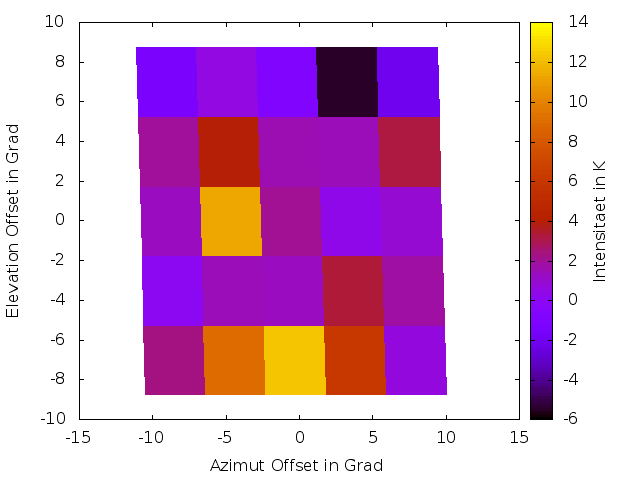
\includegraphics[width=.8\textwidth]{images/npoint_sun_color.png}
\caption{npoint Scan der Sonne mit Offset des Maximums von $2.6\, ^\circ$ Azimut und $-5.8\,^\circ$ Elevation}
\label{npoint_sun}
\end{figure}

\subsection{Cross-Scan der Sonne}
Die Daten wurden für jede Position durch Mittelwertbildung über die mittleren 48 Kanäle unter Abzug der Kalibrierungstemperatur erstellt. Die jeweils äußeren 8 Kanäle wurden nicht berücksichtigt, da die Intensität wegen der Ausleseelektronik stark abfällt. \footnote{\cite{ronomischesPraktikum}} Die Fehlerbalken zeigen die Standardabweichung dieser Mittelung.
\begin{figure}
		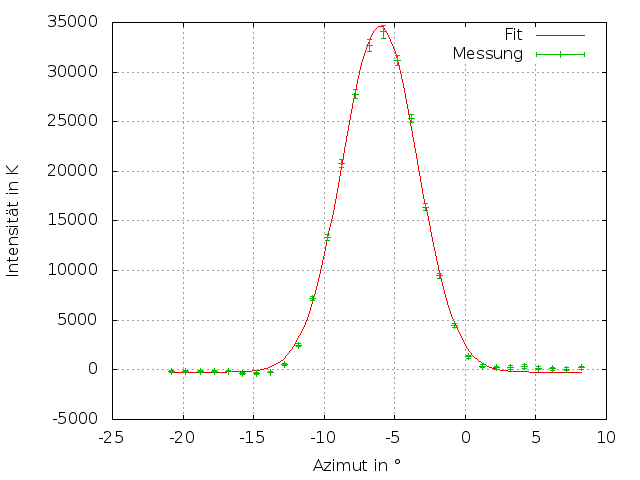
\includegraphics[width=.9\textwidth]{images/sun_azimut}
\caption{ Plot der Intensität der Sonne in Abhängigkeit des Azimutwinkels }
\label{fig:sunaz}
\end{figure}

\begin{figure}
		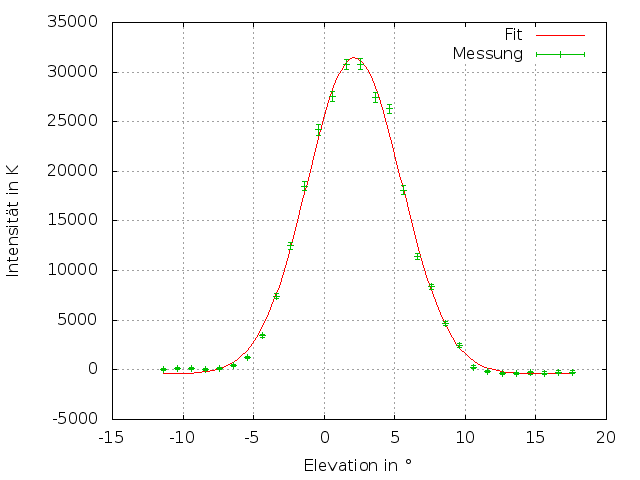
\includegraphics[width=.9\textwidth]{images/sun_elevation}
\caption{ Plot der Intensität der Sonne in Abhängigkeit des Elevationswinkels }
\label{fig:sunel}
\end{figure}

\subsection{Bestimmung der Halbwertsbreite der Antennenkeule}
Zur Bestimmung der Halbwertsbreite der Antennenkeule wurden die Messdaten mit einer Gauß-Funktion gefittet (siehe Abb. \ref{fig:sunaz} und \ref{fig:sunel}). Für die Funktion

\begin{equation}
f(x) = a \cdot e^{- \frac{(x-d)^2}{b}} + c
\label{form:FWHMfit}
\end{equation}

ergaben sich dabei Werte, wie in Tabelle \ref{tab:FWHM} zu sehen.

\begin{table}
\centering
\begin{tabular}{ccc}
Parameter	&			Wert der Azimutmessung	&	Wert der Elevationsmessung \\
\midrule
a			&			34861 $\pm$ 274			&	31855 $\pm$ 393 \\
b			&			14.32 $\pm$ 0.29		&	22.29 $\pm$ 0.72 \\
c			&			-226.4 $\pm$ 117.0		&	-401.9 $\pm$ 207.3 \\
d			&			-6.045 $\pm$ 0.023		&	2.146 $\pm$ 0.045
\end{tabular}
\caption{Werte des Fits für die Parameter aus \eqref{form:FWHMfit}}
\label{tab:FWHM}
\end{table}

Bei dieser Gauß-Funktion ergibt sich die Halbwertsbreite H folgendermaßen:

\begin{equation}
H = 2 \sqrt{2 \ln 2} \cdot \sqrt{\frac{b}{2}}
\end{equation}

Durch Fehlerfortpflanzung ergibt sich:

\begin{equation}
\delta H = \frac{\sqrt{2 \ln 2}t}{2} \sqrt{\frac{2}{b}} \cdot \delta b
\label{form:FehlerFWHM}
\end{equation}

Aus \eqref{form:FehlerFWHM} ergibt sich dann:

\begin{align*}
H_{\mr{Azimut}} = 6.300\,^\circ \ &\mathrm{und} \ \delta H_{\mr{Azimut}} = 0.062\,^\circ \\
H_{\mr{Elevation}} = 6.545\,^\circ \ &\mathrm{und} \ \delta H_{\mr{Elevation}} = 0.106\,^\circ
\end{align*}

Zusammenfassend ergibt sich also:

\begin{align}
H_{\mr{Azimut}} = 6.30\,^\circ \pm 0.07\,^\circ \\
H_{\mr{Elevation}} = 6.54\,^\circ \pm 0.11\,^\circ
\end{align}

Bei großen Elevationen führt eine Messung der azimutalen Ausdehnung der Sonne zu einer scheinbaren Verbreiterung, die dadurch hervorgerufen wird, dass das Koordinatensystem im Zenit und im Nadir Pole besitzt. Deshalb muss bei der Bestimmung der Halbwertsbreite $H_{\mr{Azimut}}$ noch mit dem $ \cos (\mr{Elevationswinkel}) $ multipliziert werden, um eine angepasste Halbwertsbreite zu erhalten. Es ergibt sich dann:

\begin{equation}
H_{\mr{Azimut,ang.}} = H_{\mr{Azimut}} \cdot \cos (30.5\,^\circ) = 5.43\,^\circ \pm 0.06\,^\circ \\
\end{equation}

\subsection{Dopplerverbreiterung durch thermische Bewegung}
Laut \cite{ronomischesPraktikum} ergibt sich die Frequenzänderung durch den Dopplereffekt aus:

\begin{equation}
\frac{\Delta \lambda}{\lambda} = \frac{v}{c}
\end{equation}
Für die thermische Bewegung bei 100 $K$ ergibt sich laut \cite{ronomischesPraktikum} eine ungefähre Geschwindigkeit von 1km/s. Damit ergibt sich:

\begin{equation}
\frac{\Delta \lambda}{\lambda} = \frac{1 \km}{2.998 \cdot 10^5 \km} = 3.34 \cdot 10^{-6}
\end{equation}

\subsection{Bestimmung der Rotationskurve der Milchstraße}
Weil das andere Teleskop während der Messung aktiviert war ergab sich ein scharfer Peak bei 1420.8 MHz(s. Abb. \ref{spektrum_beispiel}). Da sich die Störung aber au"serhalb des relevanten Bereichs befindet wurde diese Frequenzband bei der Auswertung nicht betrachtet.
\begin{figure}
    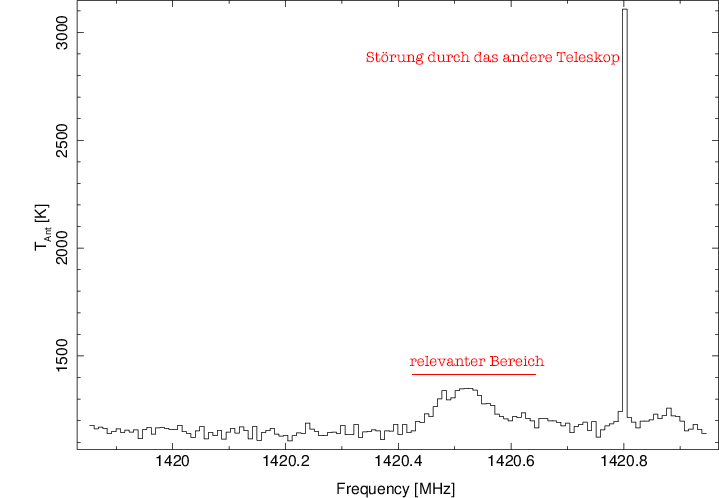
\includegraphics[width=.8\textwidth]{spektrum_beispiel.png}
    \caption{Störung durch SRT 1}
    \label{spektrum_beispiel}
\end{figure}
\begin{table}[h]
\centering
\begin{tabular}{rrrrrrr}
\multicolumn{1}{l}{l in$\,^\circ $} & \multicolumn{1}{l}{b in$\,^\circ $} & \multicolumn{1}{l}{f in MHz} & \multicolumn{1}{l}{$v_{\mr{LSR,r}}$ in km/s} & \multicolumn{1}{l}{$v_{\mr{max,observed}}$ in km/s} & \multicolumn{1}{l}{R in kpc} & \multicolumn{1}{l}{$v_{\mr{rot}}$ in km/s} \\ \midrule
0 & 0 & 1420.59 & -39.79 & 0.955 & 0.000 & 0.95 \\
5 & 0 & 1420.58 & -40.95 & 4.225 & 0.741 & 23.40 \\ 
10 & 0 & 1420.58 & -41.83 & 5.105 & 1.476 & 43.31 \\ 
15 & 0 & 1420.58 & -42.40 & 5.675 & 2.200 & 62.62 \\ 
20 & 0 & 1420.58 & -42.63 & 5.905 & 2.907 & 81.15 \\ 
25 & 0 & 1420.60 & -42.56 & 1.614 & 3.592 & 94.59 \\ 
30 & 0 & 1420.56 & -42.10 & 9.597 & 4.250 & 119.60 \\ 
35 & 0 & 1420.56 & -41.39 & 8.887 & 4.875 & 135.07 \\ 
40 & 0 & 1420.56 & -40.30 & 7.797 & 5.464 & 149.21 \\ 
50 & 0 & 1420.55 & -37.28 & 6.887 & 6.511 & 175.42 \\ 
55 & 0 & 1420.53 & -35.37 & 9.198 & 6.963 & 189.41 \\ 
60 & 0 & 1420.52 & -33.16 & 9.099 & 7.361 & 199.62 \\ 
65 & 0 & 1420.52 & -30.70 & 6.639 & 7.704 & 206.03 \\ 
70 & 0 & 1420.51 & -28.03 & 6.080 & 7.987 & 212.81 \\ 
75 & 0 & 1420.51 & -25.03 & 3.080 & 8.210 & 215.58 \\ 
80 & 0 & 1420.50 & -21.93 & 2.090 & 8.371 & 218.75 \\ 
85 & 0 & 1420.50 & -18.73 & -1.110 & 8.468 & 218.05 \\
90 & 0 & 1420.51 & -15.33 & -6.620 & 8.500 & 213.38 \\
\end{tabular}
\caption{Messtabelle mit den gemessenen Koordinaten (l,b), den Frequenzen f, die der maximalen Rotverschiebung entsprechen, den Komponenten $v_{\mr{LSR,r}}$ von $v_{\mr{LSR}}$ für die jeweilige Blickrichtung, den gemessenen Geschwindigkeiten $v_{\mr{max,observed}}$, den Abständen R zum Zentrum und den zugehörigen Rotationsgeschwindigkeiten $v_{\mr{rot}}$ }
\label{tab:Messtabelle}
\end{table}

\begin{figure}
		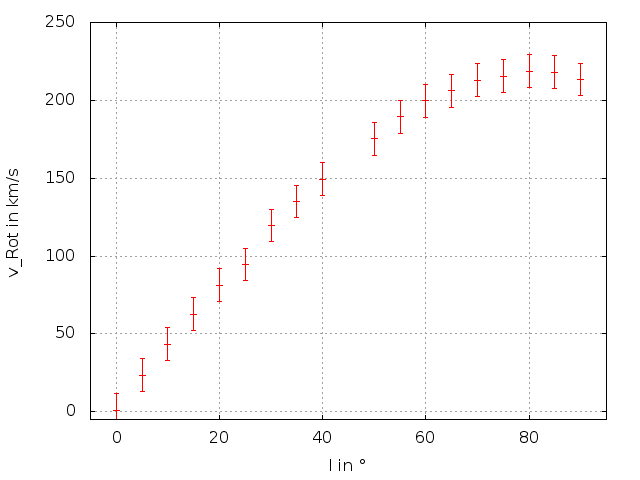
\includegraphics[width=.9\textwidth]{images/vRotberl}
\caption{ Plot der Rotationsgeschwindigkeit in Abhängigkeit des Winkels l }
\label{fig:vRot_l}
\end{figure}

\begin{figure}
		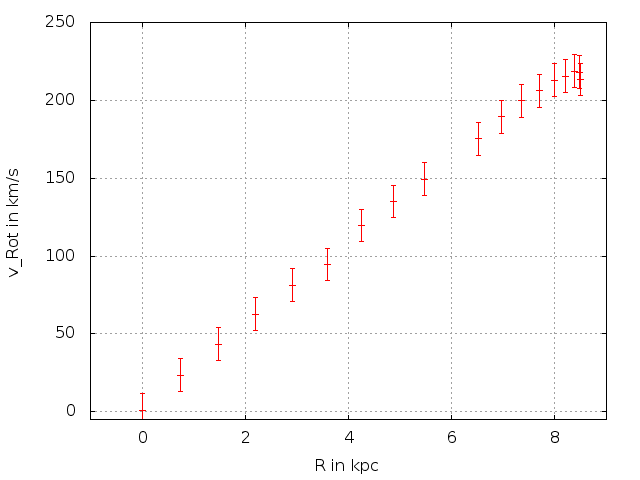
\includegraphics[width=.9\textwidth]{images/vRotberR}
\caption{ Plot der Rotationsgeschwindigkeit in Abhängigkeit des Abstandes vom Mittelpunkt der Milchstraße }
\label{fig:vRot_R}
\end{figure}

In Tabelle \ref{tab:Messtabelle} ergeben sich laut \cite{ronomischesPraktikum} die Werte aus:

\begin{align}
&v_{\mr{max,observed}} = \frac{(1420.406 \mr{MHz} - f) c}{1420.406 \mr{MHz}} - v_{lsr} \\
&R = R_0 \sin l \\
&v_{\mr{rot}} = v_{\mr{max,observed}} + \omega_0 R
\end{align}

Für $\delta v_{\mr{rot}}$ folgt mittels einer Fehlerfortpflanzung:

\begin{equation}
\delta v_{\mr{rot}} = \frac{c}{1420.406 \mr{MHz}} \cdot \delta f = 10.55 \mr{km/s} \approx 11 \mr{km/s}
\end{equation}

Daraus ergeben sich dann die Abbildungen \ref{fig:vRot_l} und \ref{fig:vRot_R}.

\subsection{Störungsmessung}
\subsubsection{Spektrum des Satelliten Afristar}
Es wurde zunächst ein npoint Scan durchgeführt um die genaue Position des Satelliten zu bestimmen. Ein Plot des Scans findet sich in \aref{npoint_afri}.
Da die Hauptfrequenz des Satelliten bei 1470 MHz liegt, ist zu erwarten, dass das Maximum des Spektrums sich auch bei dieser Frequenz befindet. Eine Darstellung der Messwerte ist in \aref{plot:afri} zu finden. Dies wird durch die Messung teilweise bestätigt. Die Werte im Bereich von 1475 bis 1500 sind teils stark negativ und scheinen von starken Schwankungen der Kalibrationstemperatur zu stammen (s. Abb. \ref{temp_afri}). Der Grund für die Schwankung konnte nicht ermittelt werden.
\begin{figure}
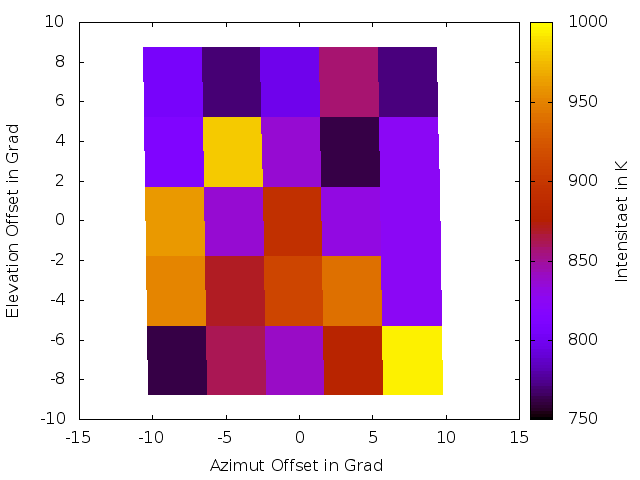
\includegraphics[width=.8\textwidth]{images/npoint_afri_color}
\caption{npoint Scan des Satelliten Afristar mit Offset des  Maximums von $7.4\,^\circ$ Azimut und $-6.0\,^\circ$ Elevation}
\label{npoint_afri}
\end{figure}
\begin{figure}
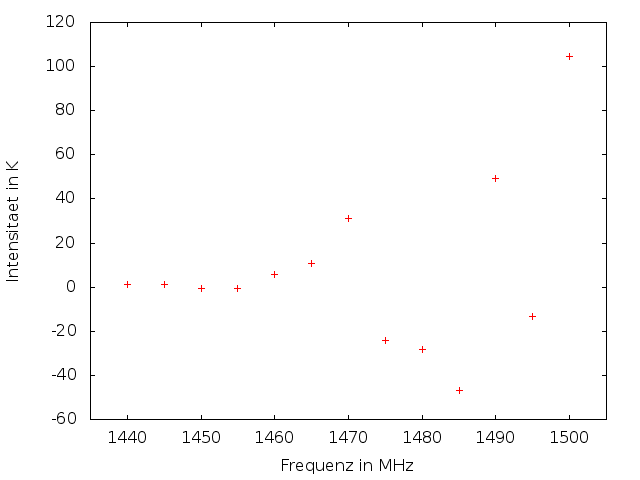
\includegraphics[width=.8\textwidth]{images/spekt_afri}
\caption{Gemessenes Spektrum des Satelliten Afristar}
\label{plot:afri}
\end{figure}
\begin{figure}
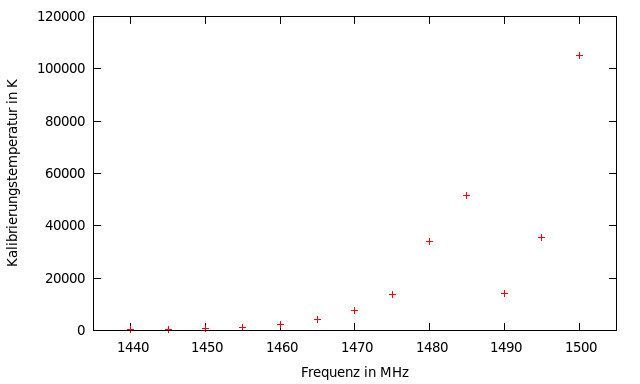
\includegraphics[width=.8\textwidth]{images/temp_spekt_afri}
\caption{Kalibrationstemperaturen aufgetragen "uber der Frequenz }
\label{temp_afri}
\end{figure}
\subsubsection{Störung durch ein Mobiltelefon}
In \aref{plot:stoer} wrude die Intensität über dem Abstand der Störquelle zum Teleskop aufgetragen. Dabei lässt sich keine vom Abstand zum Teleskop abhängige Störung feststellen. Starke Störungen traten viel mehr unvorhersehbar bei manchen Messungen auf, bei anderen blieb die Gemessene Intensität gering.
Die Unabhängigkeit der Intensität vom Abstand der Mobiltelefone ließe sich zum Beispiel durch die Verwendeten Frequenzen des Verwendeten Mobilfunkbetreibers E-Plus erklären. Die verwendeten Mobiltelefone wechseln selbstst"anding je nach Empfangsqualit"at zwischen GSM und UMTS. Dabei liegen die von diesem Provider verwendeten Frequenzen bei 880.0 - 915.0 MHz f"ur GSM\footnote{\cite{gsm}} oder bei 1935.15 - 1954.95 MHz f"ur UMTS\footnote{\cite{umts}}. 

\begin{figure}
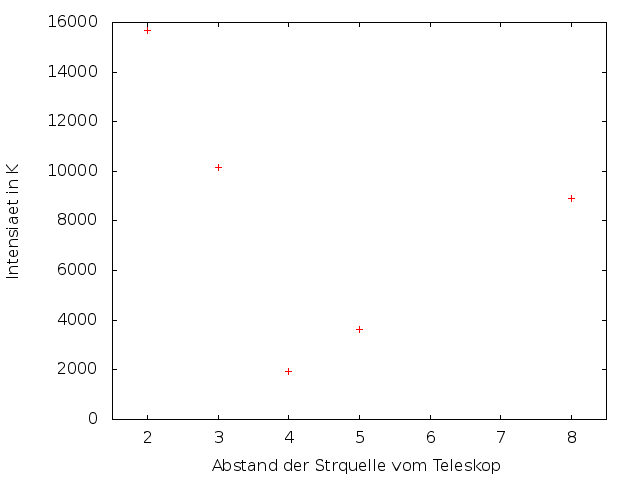
\includegraphics[width=.8\textwidth]{images/stoer}
\caption{Messung der Intensit"at bei unterschiedlicher Distanz eines Mobiltelefons zum Teleskop}
\label{plot:stoer}
\end{figure}
 
